% Please do not delete!  thanks! -- zach
% !TEX root = ../../main.tex

\section{Evaluation}
In this section, we present the evaluations that been performed on our solustions. This including two parts: 1) methods that used to evaluate our core topic learning models LDA and Doc2Vec and 2) methods used to evaluate the whole solution as the final product. 
\paragraph{Evaluating Learing Models}
The performance measure is a typical way to evaluate machine learning models. It is the measurement that will make of the predictions made by a trained model on the test dataset. Performance measures are typically specialized to the class of problem, for example in this paper, our problem is a NLP topic modeling, we will use likelihood score and perplexity to evaluate our LDA model.\\
Based on how to split the data into training and testing, evaluate machine learning models usually involves hould out, cross valiation(CV) and leave-one-out. 

\subsection{Evaluating LDA}


\subsection{Evaluating Doc2Vec}
While LDA produces keywords predicted to be the main topics of the document, Doc2Vec produces vectors. To convert these vectors in potential important topics, first the accuracy of the model must be established to ensure that it can distinguish between one topic and another. Two tests were used to evalutate the accuracy of the three Doc2Vec models, Distributed-Memory by taking the mean of the vectors (DM-M), Distributed-Memory by concatenating (DM-C), and Distributed Bag of Words (DBOW): vector prediction and information retrieval.

Doc2Vec was tested on parsed stackoverflow data. Datasets of different tags were created such that training no document in a set for one tag had any documents that contained other tags that were being tested listed. For exaple, a document tagged 'python' would not also have 'javascript' as a tag. This was done to decrease topic blending and increase the semantic importance of the tags. Tags included python, javascript, database, c\#, .net, and java. Decisions on what tags to tests, what parameters to use, etc. where decided in response to test results along the way with the goal of the models being able to distinguish a semantic difference between tags so that the models could determine which posts belonged to which tags, e.g. python post was indeed a python post and a javascript post.

\subsubsection{Information Retrieval}

One way to verify that our implementation of Doc2Vec is correctly mapping word vectors to other semantically similar word vectors is to test the trained model on an information retrieval task . \cite{RefWorks:doc:5a6e5746e4b0d609eec798d7} The data collected from stackoverflow is tagged with different topics that pertain to the content. The tags can then be used to organize the content via topic. The Doc2Vec model should report two documents that pertain to the same topic as less distant to each other than a third document that focuses on a different topic.

Three different datasets were used for this test largely based off the results of the vector prediction analysis testing: a set trained on just Python, a set trained on Python and Database, and a set trained on Python and Javascript. The Python and Javascript training data contained 25,000 randomly selected documents from each tag. Another 15,000 documetns for each tag that were not used for training were selected to be tested. Out of these 15,000 documents, two of the javascript documents were shown with one python document to determine if the model could accuratlely determine a semantic difference between the two tags allowing the model to be used for topic prediction like LDA. The same was one with the python and database set, except only 2,000 database documents were tested against 4,000 python documents shown two at a time. The rest of the python and database documents were used for training. The number database documents was far less than both python and javascript, but the database dataset scored high on the vector prediction analysis indicationg a possible semantic advantage over python and javascript. The set trained on just python was tested the same way as the other python and database set.

Mikolov et. all Used two different sources for their information retrieval tests -----CITE----. One was sentences taken from Rotten Tomatoes reviews that were labeled by MTurk workers as positive or negative. The models preformed well with being able to tell if a sentence was negative or positive, but not with five fine-tuned ratiings - if it was very positive vs. slightly positive, etc. The paragraph vector percent error for the fine-tuned ratings was a high 51.3\%. The other test involved taking 1 million popular search engine queries and creating three paragraphs several sentences long from the 10 most popular results for each query. Two of the paragraphs would be from the same source while the third would be from a different source. Their implementation of the paragraph vector was able to correctly idenity the paragraphs from the same source as closer in distance with the vector space with only a 7.42\% error. 

Similar to the fine-tuned Rotten Tomatotes experiment, attemps to implement Gensim's Doc2Vec were met with high percent errors with the parsed stackoverflow data. The error rate was determined by two measurements: the Eucildean distance and cosine simularity. Eucildean distance takes two vectors and calculates the straight-line distance between them. This measurement was used initially with poor results. The number of epochs was increased from 20 to 50 iterations in an attempt to better performance, but the error consistently became worse. The only variable that increased performance was making the number of feature vectors smaller. Upon further research, it was discovered that within a vector space, Eucildean distance is not always an accurate measurement because two vectors that are close to each other will be classified as similar even if they are going in opposite directions, thus actually being opposites in semantics. Similar semantically meaning words can also be deemed far apart if the texts vary in length greatly resulting in a high word counts creating a larger magnitude vector. Cosine simularity, the measurement Gensim uses to compare inferred vectors to the trained vectors within the models, was adopted to solve this problem.

Cosine simularity is usually used to compare vectors by the size of the cosine angle between the vector and the origin. Comparing to the origin captures the semantical direction and accounts for the magnitue problem. However, in this test the Eucildean distance consistently performed better than the cosine simularty.  ----FIGURES---  Raising epochs from 20 to 50 only seemed to affect the DM-C model, decreasing performance. The two datasets that were tested with the python and database tags performed better than python and javascript at Eucildean and cosine distance even though the python and javascript dataset was implemented with less epochs, which seemed to make the DM-C model worse. 

\subsubsection{Vector Prediction Accuracy}

One can determine how accurately the model represents the trained data by generating an inferred vector from the training corpus and comparing it to the most similar learned vector from the model. The more similar the inferred vectors of each document are to the vectors representing the same trained documents, the better the representation of the trained data. Initially, testing was done on a dataset containing both python and javascript. To avoid having to create special folders of training datasets to be used against multiple combinations of parameters, data was not chosen randomly. All of the documents in a given training corpus were used during testing. The python and javascript set was the training set created randomly before information retrieval testing that contained 25,000 posts each from python and javascript.The results from information retrieval suggested that there was not a semantic differece between python and javascript posts so python was also tested alone with all parsed python posts (slightly less than 50,000). ---FIGURE OF DATA FOR NORMAL, HIGH VECTOR, MORE EPOCHS, SMALL VECTOR)----

The results revealed several interesting points about the stackoverflow data:

-Models as a whole performec better with small 100 size feature vector. ---mostly decided by DM-C. DM-M worse. Both in python and javascript. 1st quartile and mean in DBOW very high

-DM-M performed the best with larger vectors, training more did not affect DM-M that much compared to vector size and window size. TEST 300v 20 epochs, 10 window, 50 epochs. better than window 16 at 50 epochs? 
-DM-M semi-consistent. 1-3.5 percent error. Combinining the paragraph vectors as suggested by Mikolov et all of DM-M and DBOW probably produce most consistent model good for data already trained and data that has not been seen - DM-M better at picking out topics  --> info RET.

-DM-C has the best Max when the vector was the largest - 400 neurons. More epochs ruined percent erro? TEST ABOVE. or was it the large 16 window? TEST 400v, 20epochs. best percent error when vector was small. Smaller vector = smaller vector space = less ability to determine semantic differences = better results if there is no relationship? -DBOW most consistent at percent error. Never broke .1. Good at predicting data that was already trained. Model based on probability distributions of words.
-DM-C has highest possibility for success, high maxes, but very large range, low Mins, wide 1st-3rd quartiles, low means. Probably does the best with very close semantic relationships as Mikolov suggested. They also used a combination of Dm-C and DBOW for better results. Very slow to train and did the worst with our sparce unrelated data so not worth it for this data.


-DBOW better in PYJS than just PY by .01-.02 . 20, 50-epochs not must difference. lowest at 300V 10 negative. still lower percent error than the others at other parameter changes. Consistently the best. Similar mean , quartile distribution as python. small difference between mean 1st and 3rd quartiles.


-the higher the epochs, the closer the 3rd quartile was to the max. Distance from 3rd quartile to 1st not greatly affected. Even though the percent erros would go down up with more epochs, the cosine simularities got better. Better the cosine simularity, the better the data is being represented by the model, better the topics can probably be dinstinguished? Some of the data must be very different semantically. Posts from untold amount of users on stackoverflow. 





 


\subsubsection{Conclusions}
A high error rate when trying to distinguish between topics suggests that there may be no actual semantic relationship between the stackoverflow data. Part of the problem might be the topics themselves. Python and javascript, for example, are both computer programming languages. Although they have different uses and purposes, the concepts surrounding them are more similar than say a programming language and more distance subject such as biology. To increase the semantic relationship, the stackoverflow data could be parsed more effectively. The data consisted of the 'posts' from stackoverflow. These posts did not contain the post titles or the comments. Both the titles and comment so often contain the most helpful information relevant to the topic at hand. 

Content with more specific information that is better suited for parsing could also be adopted instead. For example, typo-less information or cleaned up code from scholarly resources might allow for more efficient tokenization of relevant words or symbols like parathensis and brackets which are more prevalent in some programming languages than others. It is possible, however, that because the data from stack overflow comes from an untold amount of users, a semantic relationship may not be able to be determined. 

!!!Doc2Vec was not found to be successfull at predicting topics because of a lack of semantic relationships between datasets. Could be used to find already trained on and labeled data (VPA results) ------ If the model was accurate, could be used on pre-labeled trained data to suggest the labels from the most similar document to the inferred vector of the document being compared  --> Put in last papaer conclusion !!!!

\subsection{Evaluating Application}
\paragraph{Pre-Surveying}
To evaluate our project idea, we conducted a pre-surveying to see what the problem we are facing and how people reacting about our proposed solution. We asked our participants how long they will spend on find the right textbook, what aspect do they think is most important when choosing a textbook (except the content, our learning model will do the best of this part). See Table \ref{Pre-survey} for a breakdown of the questions to ask.

\begin{table}[ht] 
\caption{Questions in Pre-survey}
\label{Pre-survey}
\begin{center}
\begin{tabular}{ll}
\multicolumn{1}{c}{\bf Questions} 
\\ \hline \\
1. Are you a student or professor?\\
2. How much time do you spend on choosing a textbook?\\
3. How do you choose a textbook?\\
4. What aspect do you think is most important\\
when choosing a textbook (except the content)? \\
5. Would you consider an app that will give you \\
recommended textbooks base on your course \\
syllabus and your preference? \\
\end{tabular}
\end{center}
\end{table}
Among the 29 responses, we found that 73.3\% responded as they interested to our application to recommend the textbooks. The answer to most important aspect during the textbook chosen, review/ratings and sell price were the highest concern. These preliminary results give us the guidance to design the application and to improve the core learning models. See Figure \ref{result_of_presurvey} for detailed results.

\begin{figure}[ht]
\caption{Result of preSurvey}
\label{result_of_presurvey}
\centering
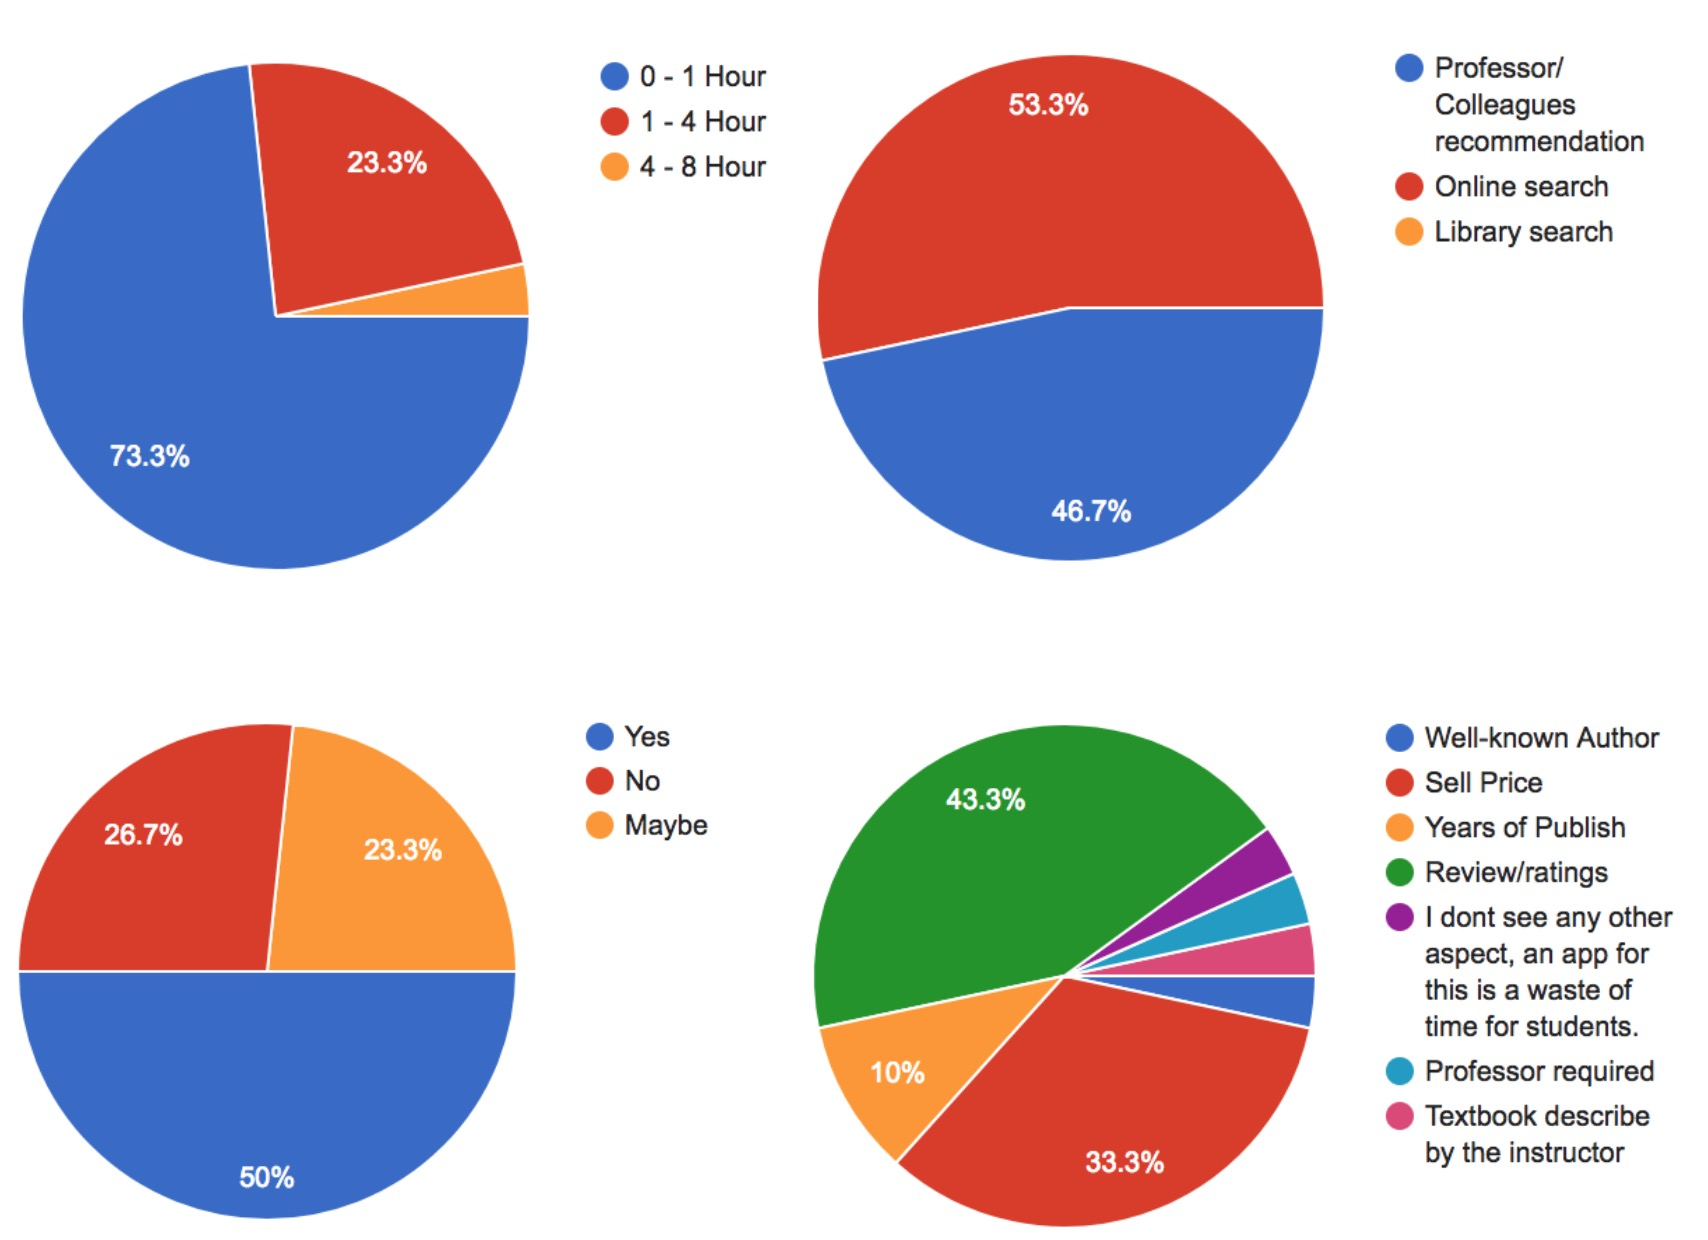
\includegraphics[width=0.5\textwidth]{preSurvey.jpeg}
\end{figure}

\paragraph{Experiments and Post-survey}
After we build the application with the command line interface and core learning models, we ran the experiments with different users in a foucs group to evaluate the solution.

%%% Local Variables:
%%% mode: latex
%%% TeX-master: "../../main"
%%% End:
